\documentclass[../BTOF_summary.tex]{subfiles}
%\usepackage{graphicx}
%\graphicspath{Pictures}
\begin{document}


\section{Calibration}

\subsection{Ongoing Performance Monitoring}

To ensure hardware component issues are detected early the system is supposed to be monitored by small LED's mounted in between the \sipms .
Short bursts of light injected into one side of the scintillator at a time will provide a stable signal source.
Changes in the measured amplitude indicates either an efficiency loss in the scintillator or a gain drop of the involved \sipms .
These signals also act as a reference point in order to determine the time resolution of the detector elements while they are deployed.

It is foreseen to have four channels for all the LED's on one \railboard .
This allows for every other LED on a single side along the board to be illuminated, leaving a dark scintillator between two illuminated scintillators.
This ensures the signal is only produced by the internal light with no light bleed from a neighboring tile.
By only illuminating one side \todo{what is the benefit of this?}

This method needs to be improved as tests have shown that the signals measured from both sides of the scintillator tile vary in intensity, although it was assumed that these LEDs would be used for accurate measurements.
Figure ~\ref{fig:TD} shows a time delay measurement.
Further, for calibration, we used such signal sources as Sr-90, Na-22, and a laser.

\begin{figure}[h!]
    \centering
    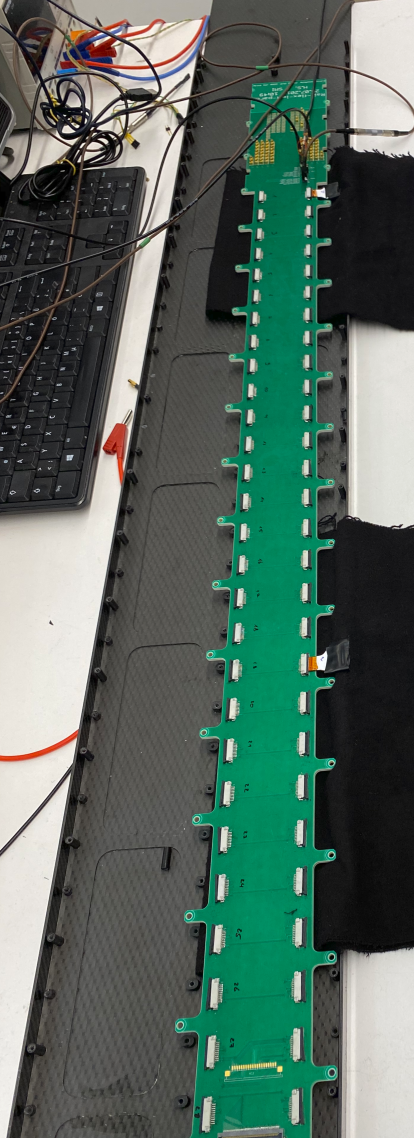
\includegraphics[scale=0.2, angle =270]{Pictures/pic1.png}
    \caption{Figure 1: Tests with two LEDs on the board 1: signals measured at odd connectors 1 and 19 on the left side.}
    \label{fig:TD}
\end{figure}

\subsection{Position Calibration}

In order to deliver useful position information for the detector hits the exact position of each tile in the context of the detector needs to be determined.\unsure{this is probably done by in the commissioning phase of the detector setup for the whole experiment.}
The position of the individual scintillator tiles is mainly of interest in the context of the time resolution, signal delay and amplitude drop along the board which are discussed in the following sections.

\subsubsection{Time Resolution Expectancy along the Board}

Since the time resolution is affected by signal noise and decreases of the slope of the rising flank it can be expected to receive a worse time resolution for scintillators farther down the \railboard\ with a longer distance between the detector element and the Front End Electronics.
In order to create a baseline for the detector performance the time resolution needs to be measured along the length of the \railboard .
A pulsed signal with a frequency of 50 kHz, 5 V and a duration of 20 ns from a signal generator is used to power the laser diode. The light signal is transmitted through an optical fiber to the middle of the scintillator plate, which is located inside the plastic box (see Fig.~\ref{fig:Box_SciTile},~\ref{fig:Box_SciTile1}). The box protects SciTil from outside light and moves very neatly across the \railboard.
Measuring the time of flight variation, which is expressed by the standard deviation, at each slot along the entire \railboard\ gives fairly similar good results in the 90 to 160 ps range (or double the time resolution of the scintillator) (see Fig. ~\ref{fig:TR}), but the time difference between the two signals increases on the second part (see Fig. ~\ref{fig:Diff}, shown for the left part of the board) of the railboard due to waveform distortion (reflections, different signal attenuation on two sides of one slot).

\begin{figure}[h!]
   \centering
    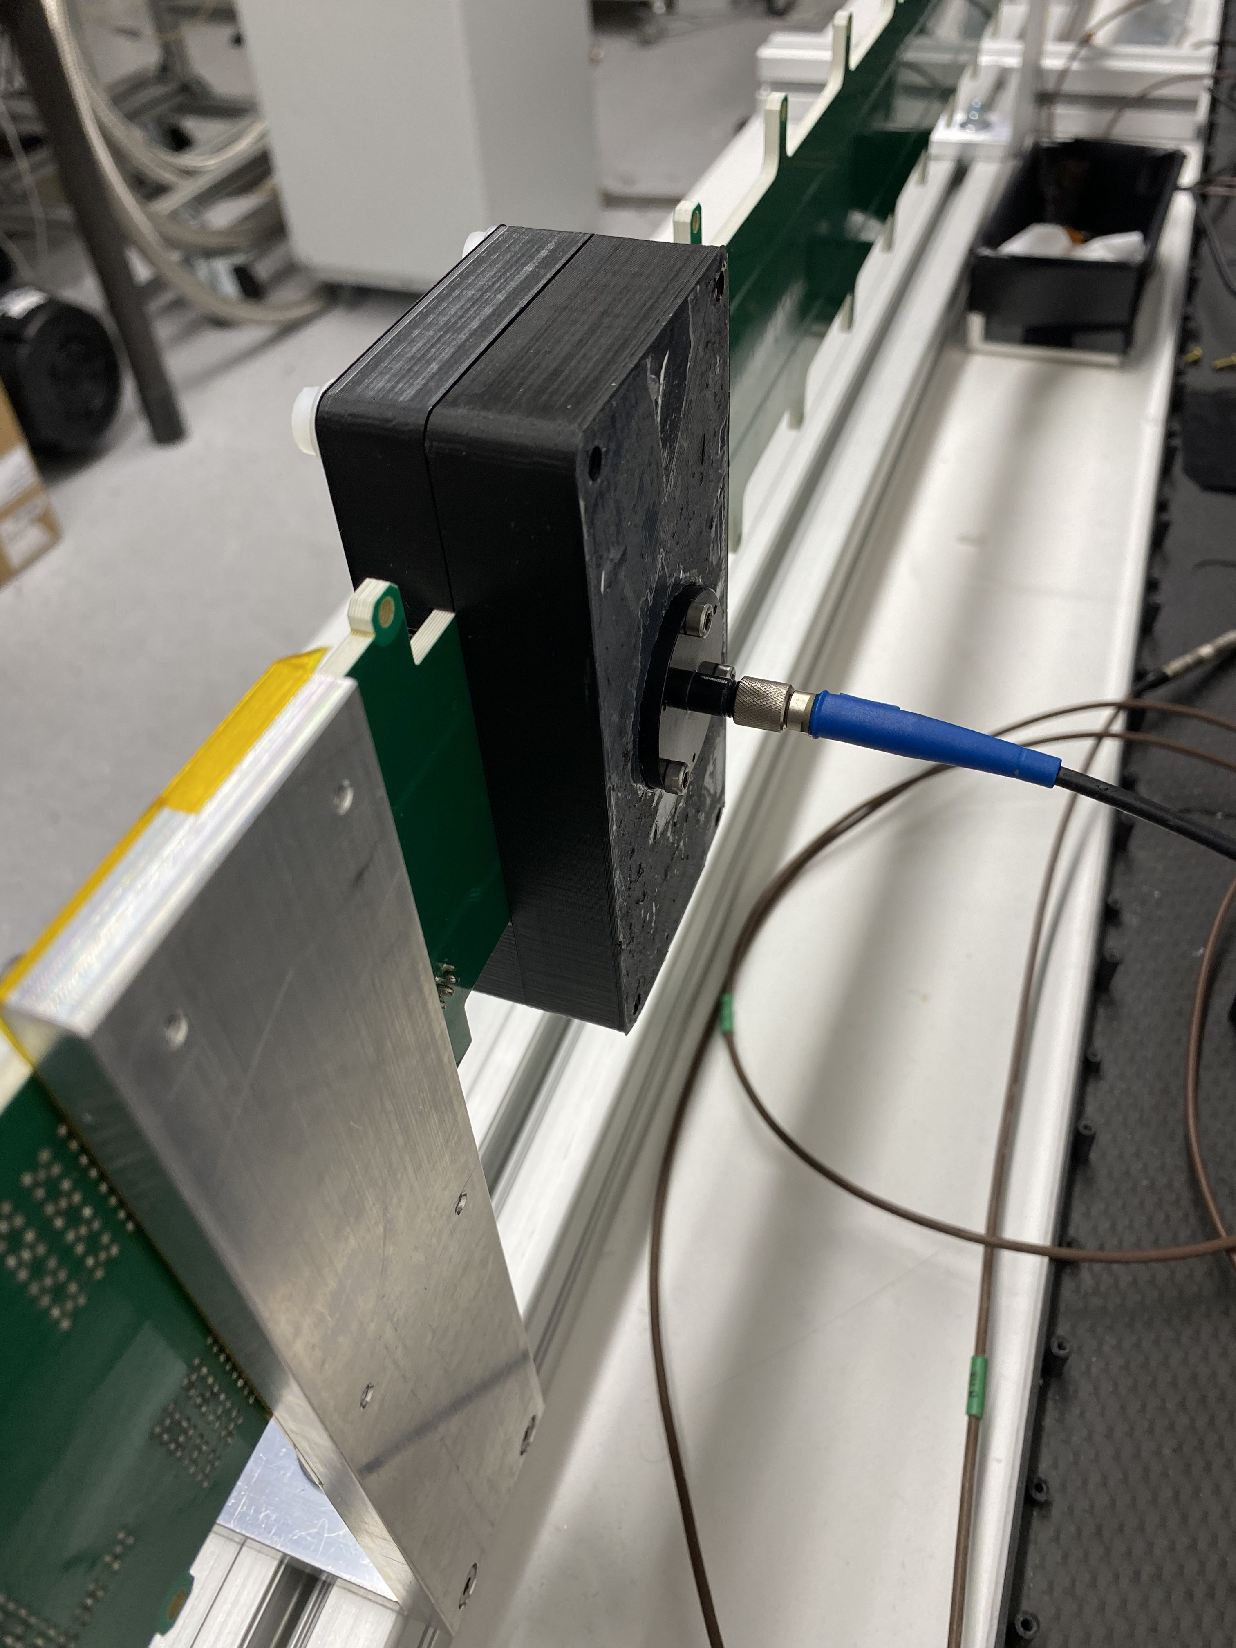
\includegraphics[scale=0.2]{Pictures/Box_SciTile.pdf}
    \caption{Experimental setup: a black plastic box is attached to the railboard. The light signal is transmitted through an optical fiber.}
    \label{fig:Box_SciTile}
\end{figure}

\begin{figure}[h!]
    \centering
    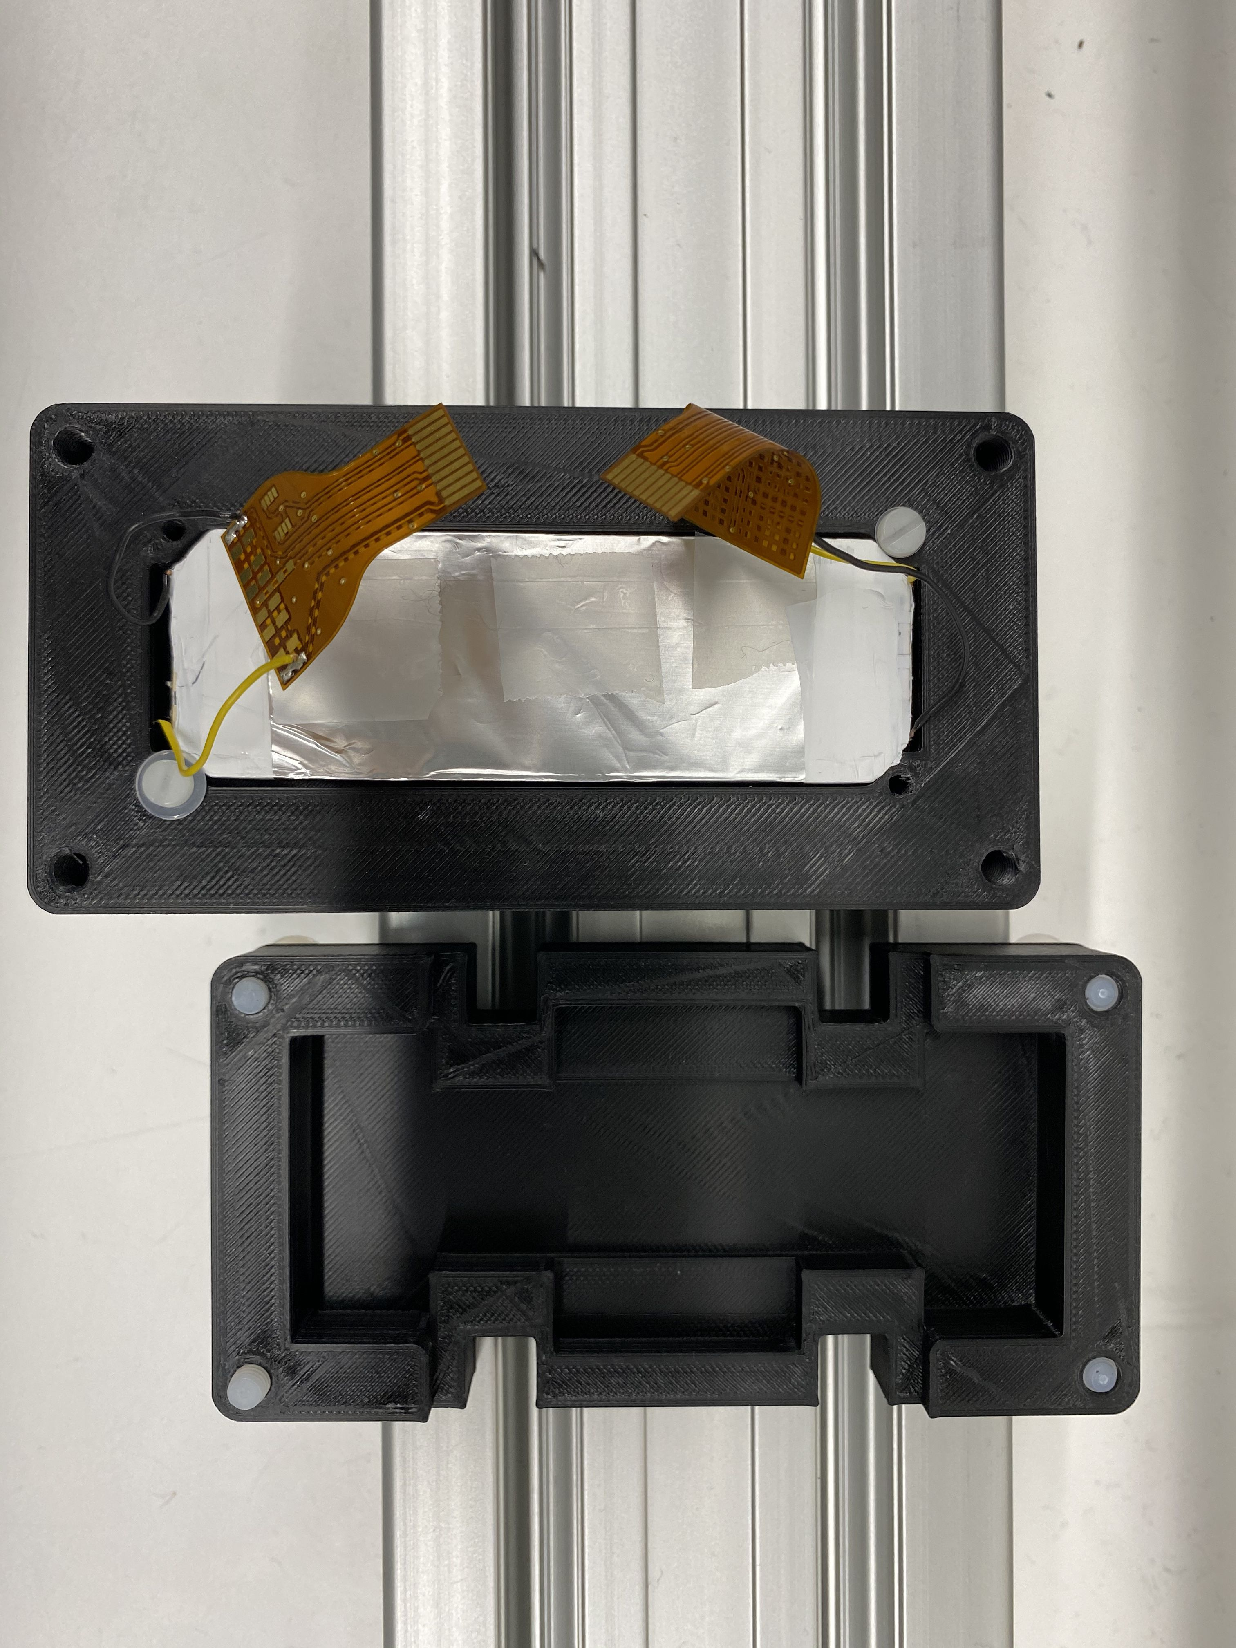
\includegraphics[scale=0.2, angle=90]{Pictures/Box_SciTile1.pdf}
    \caption{The scintillator plate is located inside the plastic box, the flexible Sensor-Board is soldered with short wires to the photodetectors.}
    \label{fig:Box_SciTile1}
\end{figure}

\begin{figure}[h!]
    \centering
    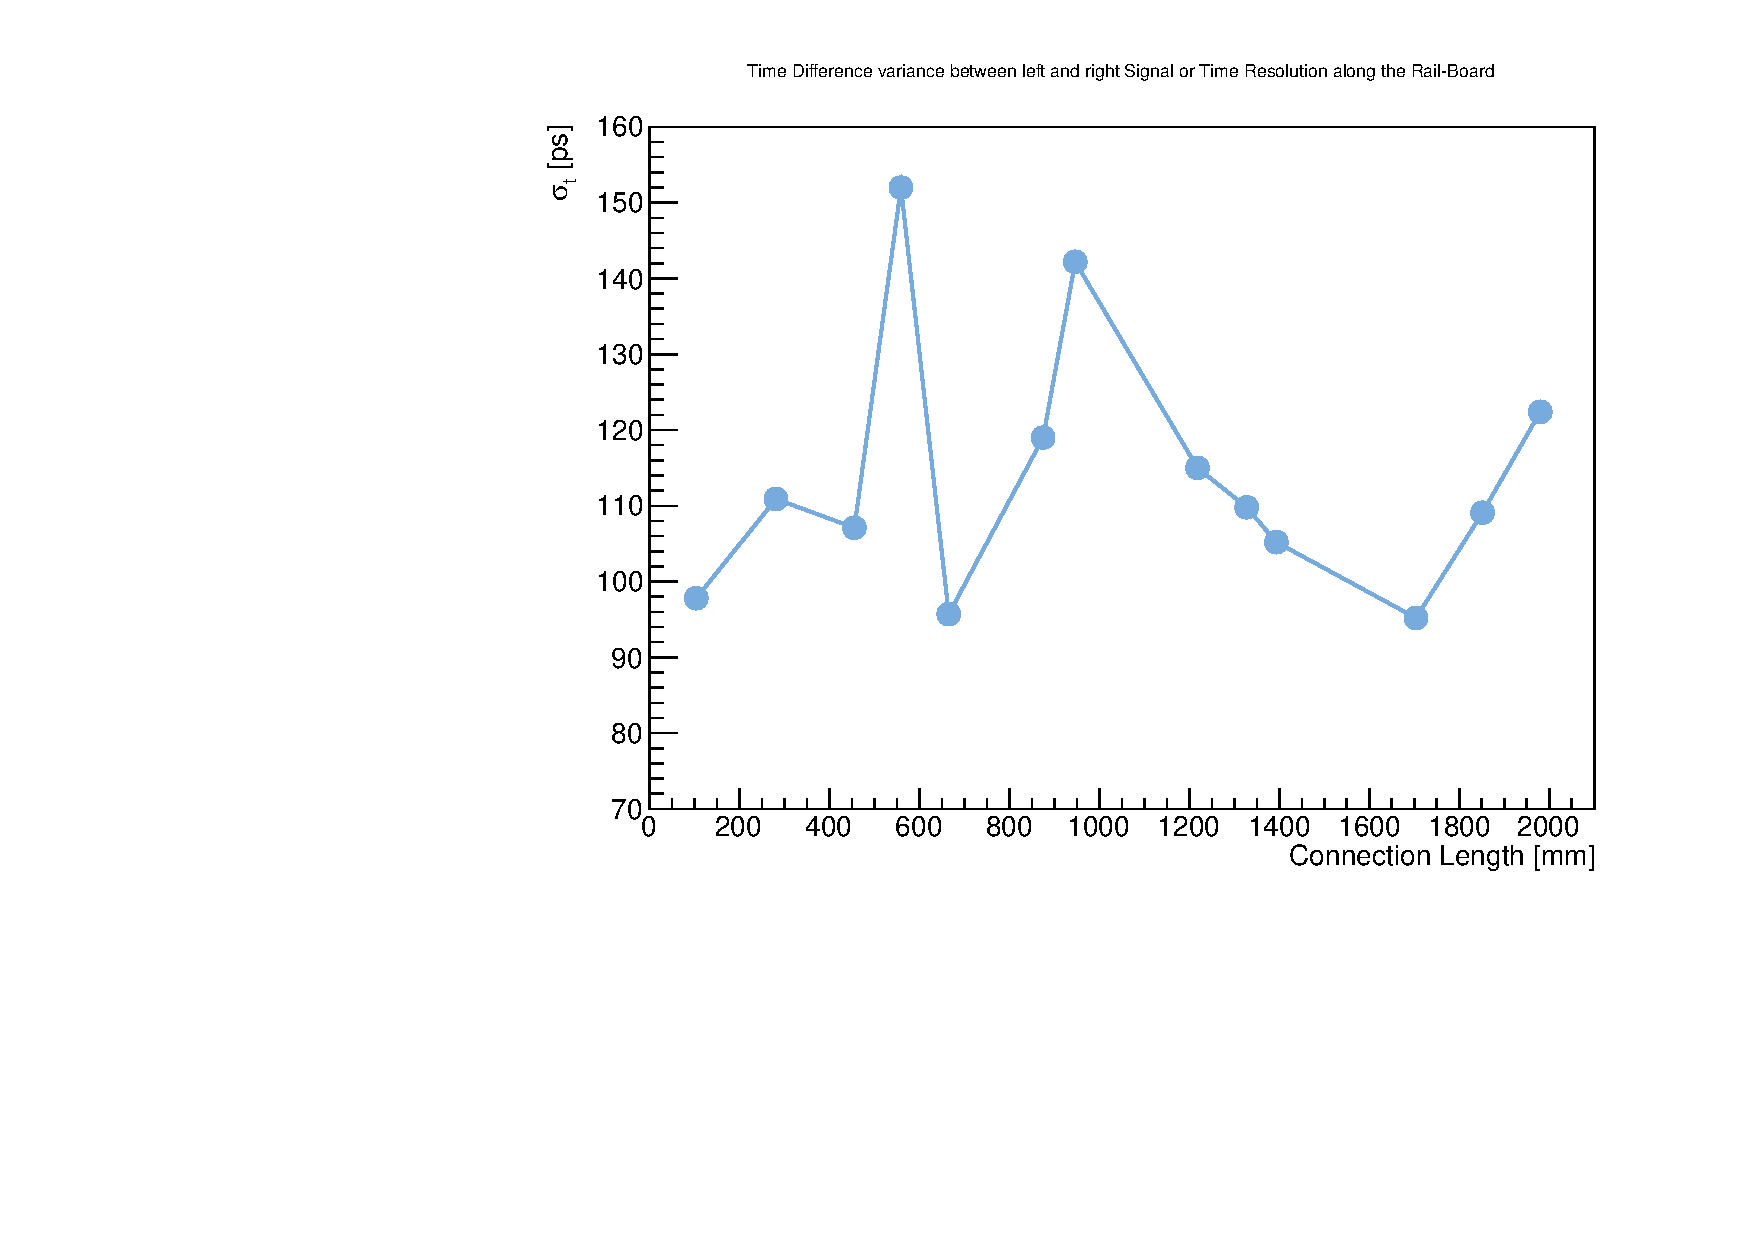
\includegraphics[scale=0.5]{Pictures/TimeRes.pdf}
    \caption{The measured time difference resolution.}
    \label{fig:TR}
\end{figure}

\begin{figure}[h!]
    \centering
    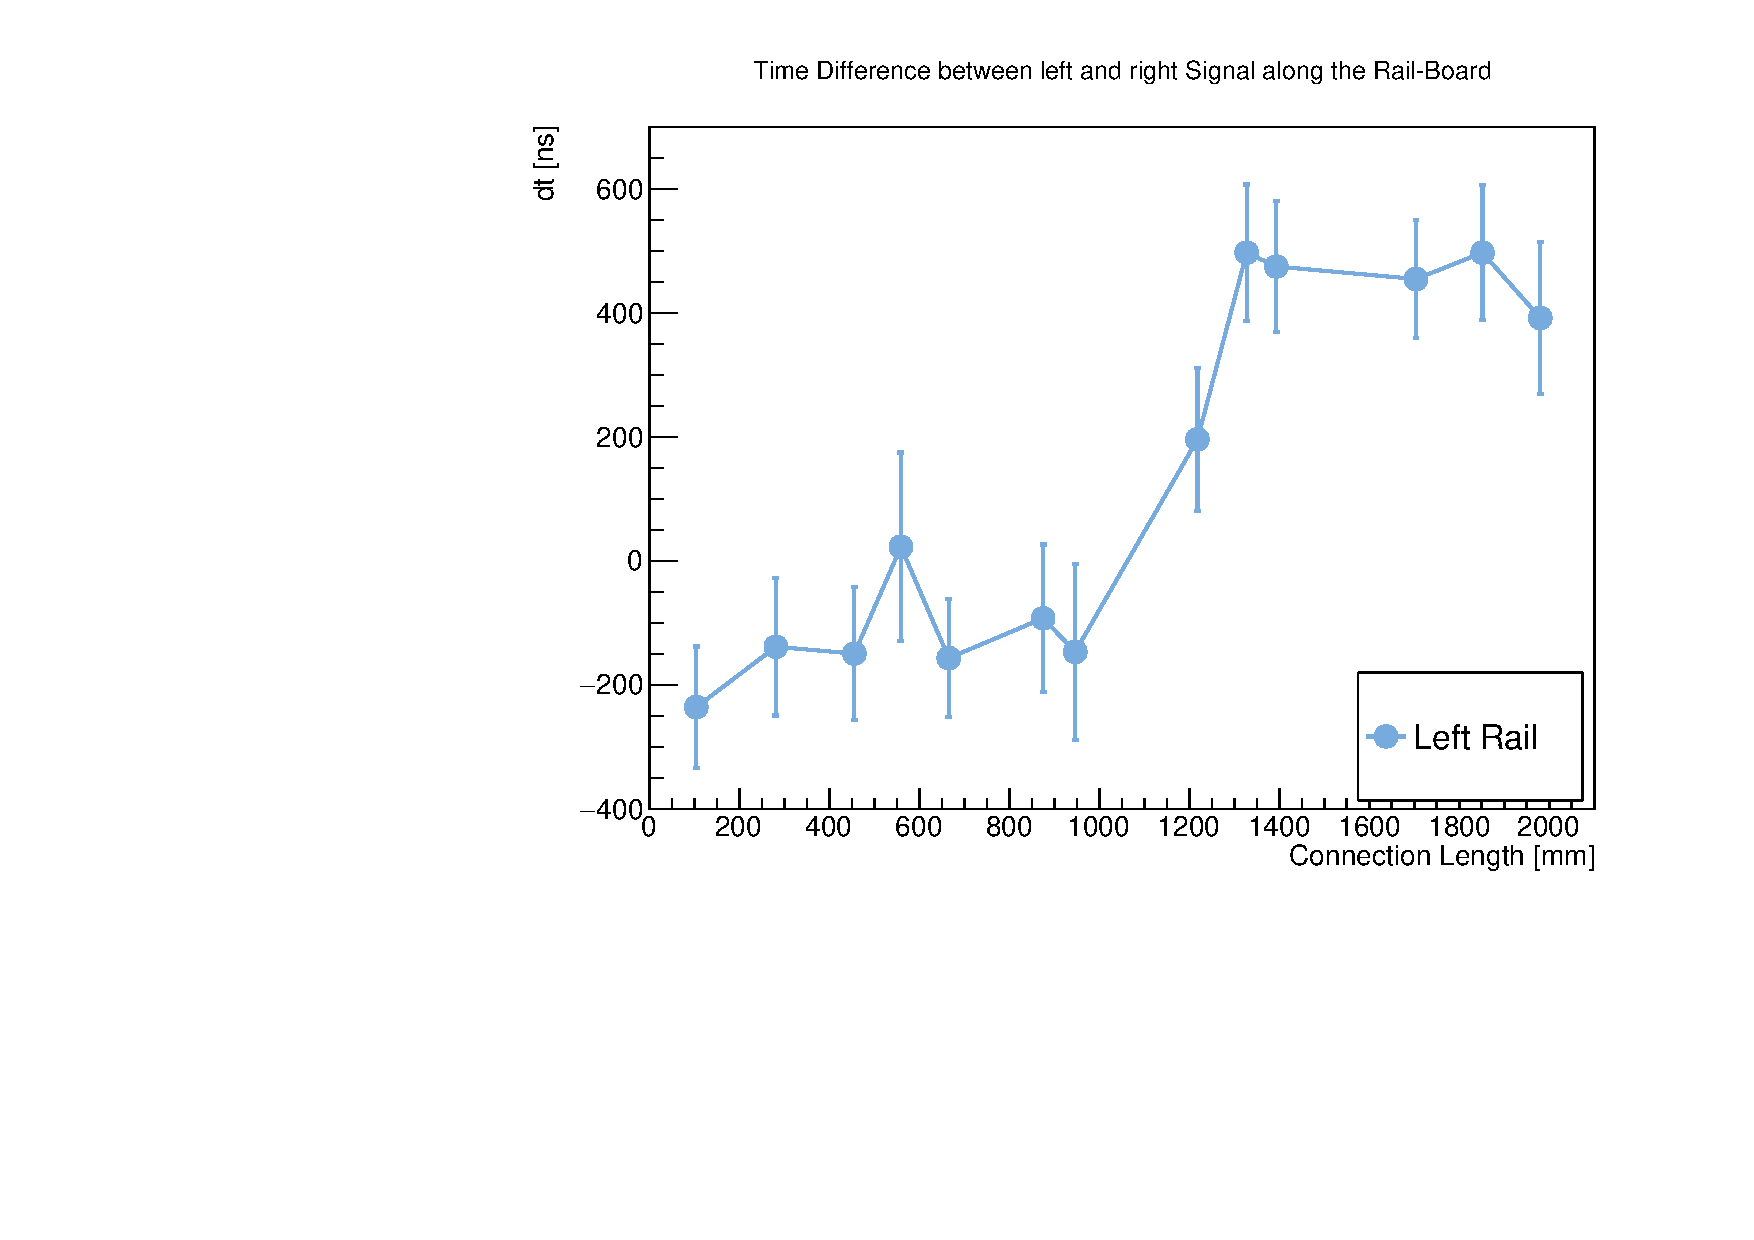
\includegraphics[scale=0.5]{Pictures/TimeDiff_leftRight.pdf}
    \caption{Time difference between the left and right SiPM arrays signals, measured in the middle of the scintillation plate.}
    \label{fig:Diff}
\end{figure}

\subsubsection{Signal Delay along the Board}

In order to provide an accurate time stamp for hits in the \btofD\ the time a signal needs to travel from the \sipms\ to the FEE has to be taken into account. The longer the electrical connection line is the larger the time delay between detector hit and time stamp in the electronics.

The speed a signal travels through a copper connection is significantly slower than the speed of light.

Comparing the accumulated signal latency over the entire length of the board (between slots 1 and 60) with what we should expect from theory, that is, the signal velocity is usually about 16.3 cm per nanosecond \cite{bril,paul}, which shows a good match (see Fig. ~\ref{fig:DiffTr}).

\begin{figure}[h!]
    \centering
    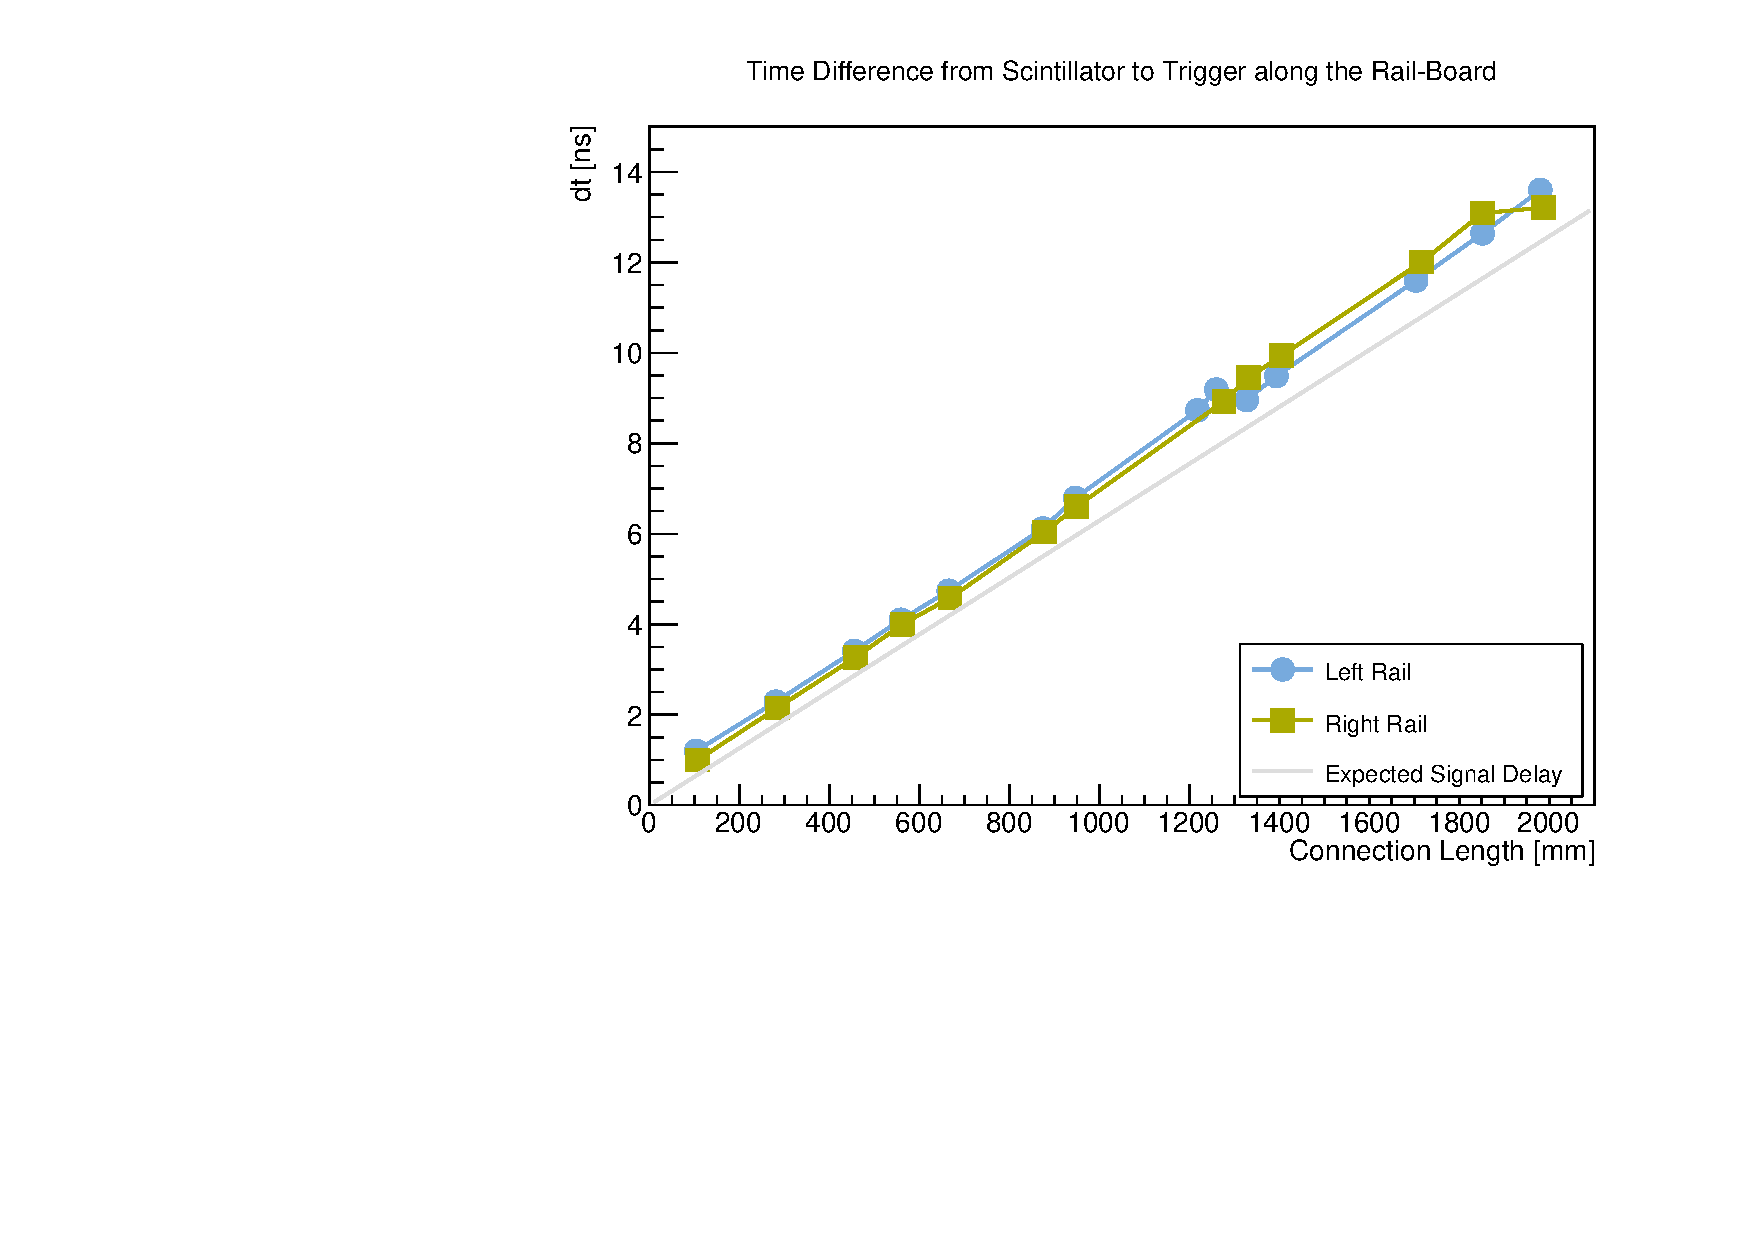
\includegraphics[scale=0.5]{Pictures/TimeDiff_toTrigger.pdf}
    \caption{Time difference between the signals from the left (blue) SiPM arrays and the right SiPM arrays (green) and the reference signal (trigger), measured in the middle of the scintillation plate along the \railboard.}
    \label{fig:DiffTr}
\end{figure}

\subsubsection{Amplitude Drop along the Board}
Signal attenuation measurements have shown that a drop of up to 23\% is expected for an internal connection of 2m length, which means a fairly strong amplitude drop (see Fig. ~\ref{fig:SA}).

\begin{figure}[h!]
    \centering
    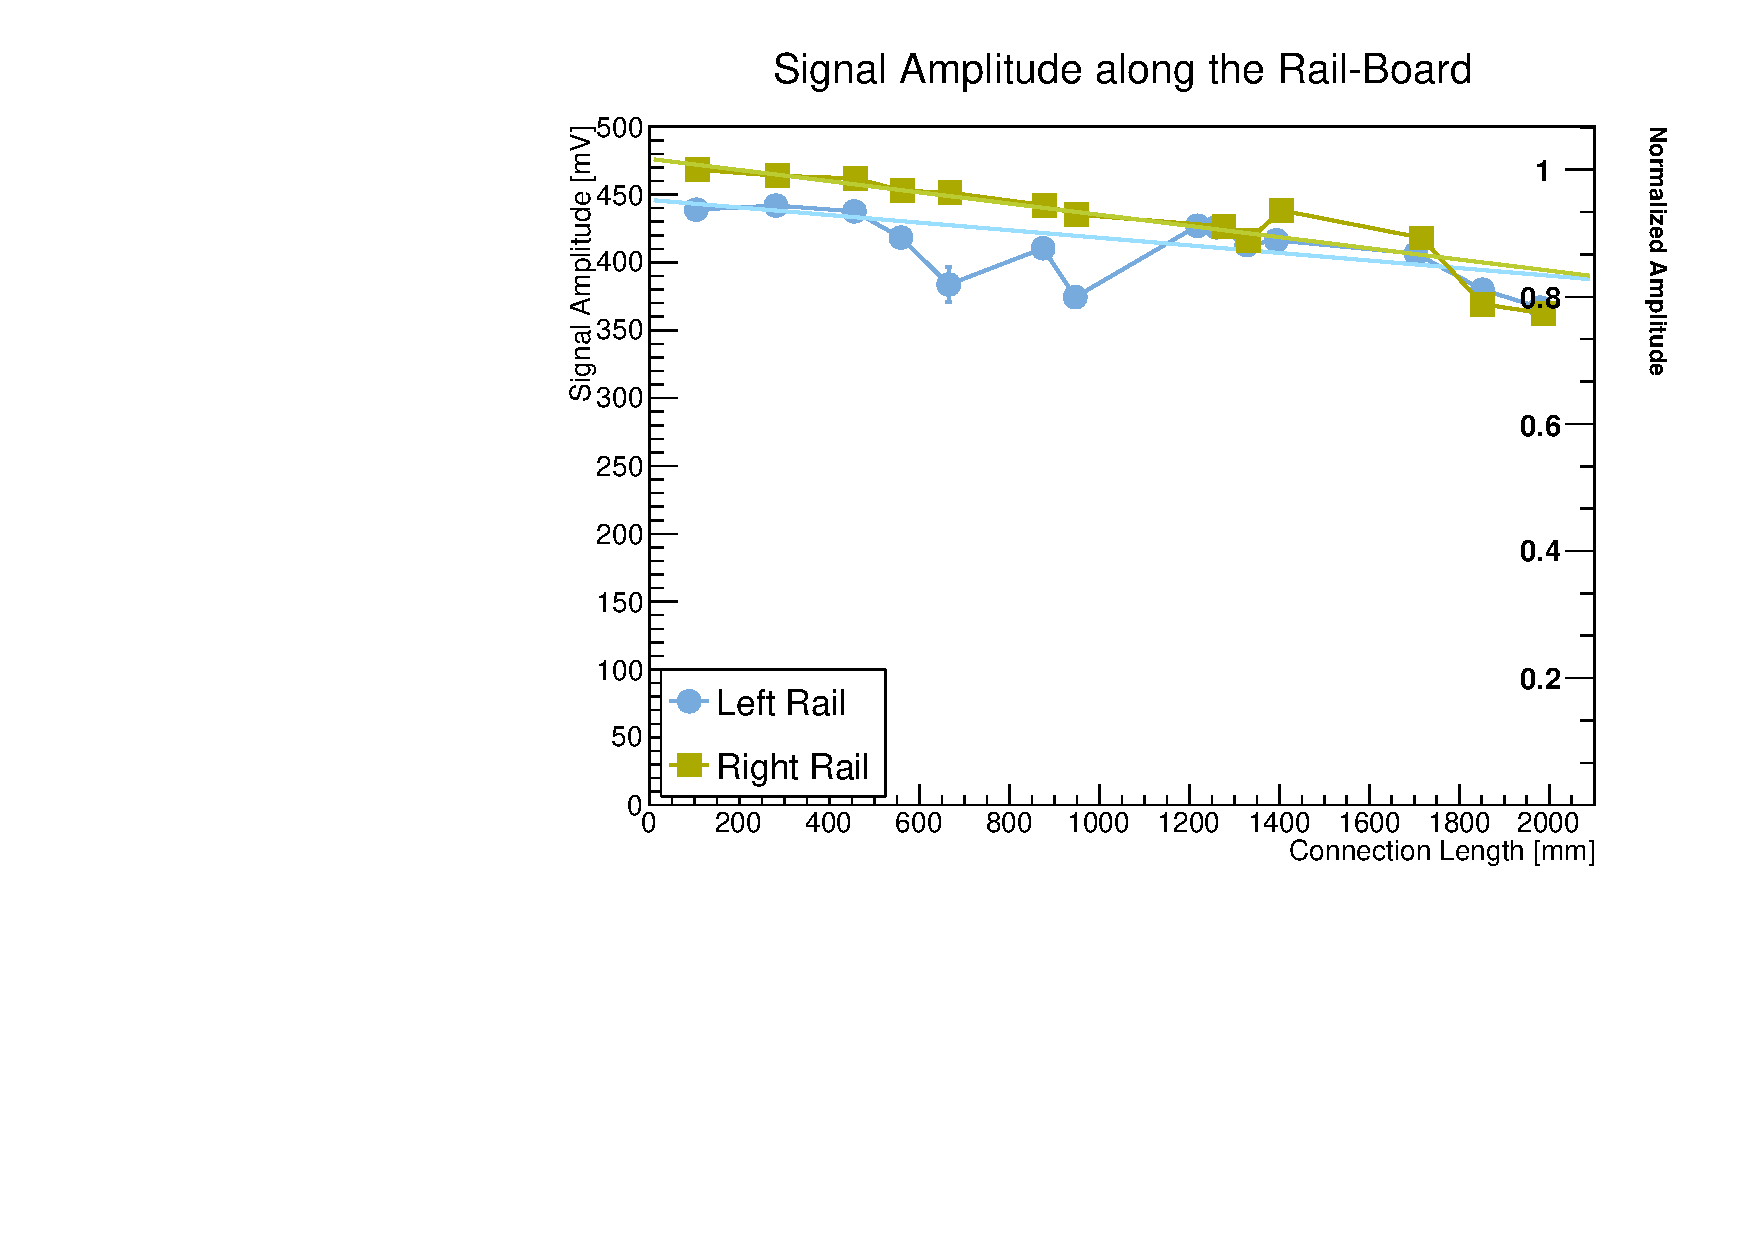
\includegraphics[scale=0.5]{Pictures/SignalAmplitude.pdf}
    \caption{Signal amplitude drop measured along the staff: a drop of up to 23\% is expected for an internal connection of 2 m length.Two strong drops with amplitude measured at 650 mm (slot 20) and 950 mm (slot 30) on the left side are due to mechanical squeezing the flexible Sensor-Board.}
    \label{fig:SA}
\end{figure}



From the measurement results, the following conclusions were drawn from a technical point of view:

1. Flexible PCBs, along with ease of use on the one hand, showed waveform distortion when bent, on the other hand.

2. In order to prevent the rapid destruction of the PCB with repeated bends due to the fragility of the wiring, the tests used the connection of the PCB with photodetectors using short wires.

3. Connectors along the boards for reading signals are reliable and convenient, gold connectors for read-out are also quite reliable, but not very firmly attached to the board.

4. External light affects measurements. In order to minimize this influence, the test setup was equipped with an insulating box.

5. There was no apparent jump in amplitude when switching from one board to another, associated with electrical connections, although signal distortions due to mechanical deformations of the ribbon cable (to ensure the connection of two boards) and the PCB occurred frequently, which led to a noticeable drop in amplitude.

6. Signal measurements on the second board showed an inconsistent signal amplitude change, likely related to the electrical wiring diagram.

\begin{thebibliography}{9}
\bibitem{bril} 
Brillouin, Léon. 
\textit{Wave propagation and group velocity}. 
Academic Press Inc., New York, 1960.

\bibitem{paul} 
Clayton R. Paul. 
\textit{Analysis of Multiconductor Transmission Lines}. 
Johm Wiley \& Sons., New York, 1994.

\end{thebibliography}
\end{document}
